\documentclass[conference]{IEEEtran}

\usepackage{cite}
\usepackage{amsmath,amssymb,amsfonts}
\usepackage{verbatim} % um viele zeilen auszukommentieren
\usepackage{algorithmic}
\usepackage{listings}
\usepackage{listings}
\lstset{
	language=Python,
	basicstyle=\ttfamily\small,
	aboveskip={1.0\baselineskip},
	belowskip={1.0\baselineskip},
	columns=fixed,
	extendedchars=true,
	breaklines=true,
	tabsize=4,
	frame=lines,
	showtabs=false,
	showspaces=false,
	showstringspaces=false,
	keywordstyle=\color[rgb]{0.627,0.126,0.941},
	commentstyle=\color[rgb]{0.133,0.545,0.133},
	stringstyle=\color[rgb]{01,0,0},
	numbers=left,
	numberstyle=\small,
	stepnumber=1,
	numbersep=10pt,
	captionpos=t,
	escapeinside={\%*}{*)}
}


\usepackage{graphicx}
\usepackage[ngerman]{babel}		% Achtung umlaut 
\usepackage[utf8]{inputenc}       % UTF-8 ist wichtig,  ASCII hat nicht alle Schriftzeichen  
\usepackage{textcomp}
\usepackage{xcolor}
\usepackage{dirtytalk} % nein, nicht was du denkst.  Packet hilft  gegen verschluckte gänsefüschen
\def\BibTeX{{\rm B\kern-.05em{\sc i\kern-.025em b}\kern-.08em T\kern-.1667em\lower.7ex\hbox{E}\kern-.125emX}}
\begin{document}


\title{Projekt rosBerry *\\
{\footnotesize \textsuperscript{*}Ein Autonomer Roboter auf Basis von ROS, gebaut aus einem Modellauto Chassis mit Maker Elektronik}}

\author{\IEEEauthorblockN{1\textsuperscript{st} Welter, Heike}
\IEEEauthorblockA{\textit{Hochschule Mannheim} \\
1630298@stud.hs-mannheim.de}%
\and
\IEEEauthorblockN{2\textsuperscript{nd} Matheis, Steffen}
\IEEEauthorblockA{\textit{Hochschule Mannheim} \\
1712806@stud.hs-mannheim.de }
\and
\IEEEauthorblockN{3\textsuperscript{rd} Barsalou, Marie }
\IEEEauthorblockA{\textit{Hochschule Mannheim} \\
1611347@stud.hs-mannheim.de}
}

\maketitle

\begin{abstract}
Ziel von Projekt rosBerry besteht darin, einen kleinen, schnellen aber dennoch preisgünstigen Roboter aus leicht verfügbaren Standardbauteilen zu bauen.
Zusätzlich soll er mit dem Robot Operating System betrieben und mit einer Künstlichen Intelligenz versehen werden.
Der Roboter soll einen optischen Marker erkennen und darauf zufahren.
Frontalzusammenstöße mit Wänden soll er dabei vermeiden.
\end{abstract}

\begin{IEEEkeywords}
Roboter, ROS, KI, Raspi, Neuronale Netze, Arduino
\end{IEEEkeywords}

%\section{Einleitung }  wollen wir  eine machen?
%projekteinleitung text hier
\section{Theorie zu Roboter und seiner Künstlichen Intelligenz}

\subsection{Vergleichbare Projekte}	%mary
Wenige Projekte der Robotik oder der Künstlichen Intelligenz für Autonome Systeme existieren, ohne das es nicht andere vergleichbare Projekte gibt.
\\

\subsubsection{Vergleichbare Hardwareansätze — Donkey Cars} %mary
%Donkey car infos
Die Hardware des Roboters wurde vom Donkey Car Projekt inspiriert.
Das Donkey Car Projekt beschäftigt sich damit, ein ferngesteuertes Auto mit einem Raspberry Pi zu steuern.
Mehr Informationen zu diesem Projekt gibt es auf ihrer Website https://docs.donkeycar.com.
Donkey Cars fahren größtenteils mit Hilfe von quelloffenem Python Code. \\
\\
Auf Youtube hat ein Benutzer namens Tiziano Fiorenzani gezeigt, wie ein Donkey Car mit ROS betrieben werden kann.
Das Video https://youtu.be/iLiI\_IRedhI verweist auf Github für Tiziano Fiorenzanis Code.
Das Projekt wurde um einen Arduino und mehrere ROS Nodes erweitert.
% Tiziano der Rasende Italiener auf youtube

\subsubsection{Vergleichbare Projekte zur Künstlichen Intelligenz} %steffen ? mary?
Das Neuronale Netz zur Bildklassifizierung ist an das Buch \glqq Artificial Intelligence for Robotics\grqq  \cite{b1} angelehnt.
Darin vermittelt F. Grovers wie Künstliche Intelligenz für Autonome Systeme funktionieren kann, indem er zeigt wie er einem kleinen Roboter beibringen würde aufzuräumen.
In einem Kapitel beschreibt der Autor, dass der Roboter mit Hilfe von Neuronalen Netzen lernen soll ob sich Spielzeuge auf dem Teppich befinden, um sie später aufzuräumen.
Da unserer Anwendungsfall ein anderer ist, musste die Datenmenge erhöht werden, das Neuronale Netz wurde erweitert und die Auflösung des Bildes wurde erhöht.
\\

Auch die Bachelorarbeit \glqq Bildklassifikation auf einem Raspberry Pi Zero am Beispiel einer Ladestationserkennung\grqq \cite{b2} von Amanda Decker ist ein vergleichbares Projekt.
Einige der Grundansätze aus dieser Arbeit wurden für dieses Projekt übernommen.
So haben wir das Neuronale Netz nicht auf einem Raspberry Pi trainiert und einen Marker genommen der sich gut rotieren und spiegeln lässt.
Somit kann jedes Bild des Datensatzes gespiegelt werden, um mit mehr Daten arbeiten zu können.
Anders als Amanda Decker jedoch haben wir uns für Keras entschieden, statt eine selbstgeschriebene Künstliche Intelligenz zu verwenden.

\section{Theoretische Grundlagen von Projekt rosBerry}

\subsection{Neuronale Netze in Theorie}	%steffen

\subsection{Ansätze für die Erstellung vom Datensatz}	%mary

Bei Amanda Deckers Bachelorarbeit schien die KI Schwierigkeiten damit zu haben zwischen dem Marker und einem Blauton zu unterscheiden, der auch im Marker vorkam.
Es schien auch schwierig zu sein ein Binärbild vom Marker zu erzeugen, da die beiden Farben des Markers einen geringen Kontrast zueinander haben.
Da Kameras in Opencv mit Hilfe von Schachbrettmustern kalibriert werden, wird für dieses Projekt ein Symbol mit ähnlich hohem Kontrast und scharfen Kanten verwendet.
\\
%Marker Bild hier? Unbedingt!
Dieses Symbol ist nicht nur in 4 Richtungen rotierbar, sondern auch zweifach spiegelbar, ohne den Marker zu verfälschen. (Rotationsinvarianz und Spiegelungsinvarianz)
Es verfügt auch über einen maximalen Kontrast und klare, gerade Kanten.
\\
\noindent
Ein Neuronales Netz kann nur so gut sein wie die Daten, mit denen es trainiert und getestet wurde.
In vielen wissenschaftlichen und populärwissenschaftlichen Artikeln wurde beschrieben, wie ein ungeeigneter Datensatz zu unbrauchbaren Ergebnissen führte.
So wurden Vorurteile der Forscher bestätigt, oder die KI traf Entscheidungen anhand von falschen Kriterien, wie der Bildunterschrift statt des Bildinhalts.
\\
Um einen möglichst robusten Datensatz zu bekommen werden verschiedene Techniken angewendet:
\begin{itemize}
	\item Um zu verhindern, dass die KI alle Bilder mit starken Kontrasten für einen Marker hält, wird ein Ausschnitt einmal mit und einmal ohne den Marker fotografiert.
	\item Gegen den \glqq schön-wetter KI\grqq-Effekt (eine KI die annimmt jedes gut ausgeleuchtete Bild muss ein Treffer sein) wird der Marker bei verschiedenen Beleuchtungen fotografiert.
	Dazu gehören direktes Sonnenlicht, Schatten, künstliche Beleuchtung mit LED, Lampen und Neonröhren. 
	\item Um zu verhindern, dass die KI alles für ihren Marker hält, was eine gewisse Größe hat und quadratisch ist, wurde der Marker aus verschiedenen Distanzen fotografiert. 
	\item Gegen Noise Anfälligkeit wurden verschiedene Hintergründe bei den Fotos verwendet. Teils weiße Wände, teils strukturierte Hintergründe oder eine Freifläche. 
	\item Um zu verhindern das sich die KI auf die Bildmitte konzentrieren kann wird der Marker aus verschieden Positionen fotografiert. 
\end{itemize}

% bilder ++
% wie unterschiedliche bilder
\subsection{Grobübersicht über das System}
In diesem Kapitel werden wir, bevor wir näher auf die Softwarearchitektur und den Hardwareaufbau von rosBerry eingehen, das System kurz als Gesamtüberblick vorstellen.

\begin{figure}[!ht]
	\centering
	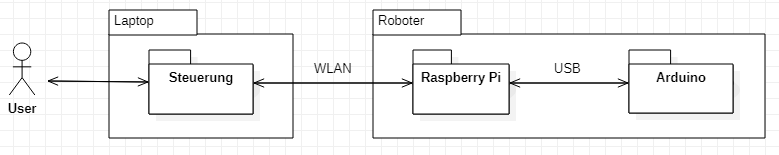
\includegraphics[width=9cm]{img/Gesamtsystem.PNG}
	\caption{Gesamtüberblick des Systems}
	\label{Gesamtzusammenhang}
\end{figure}
Die Abbildung \ref{Gesamtzusammenhang} zeigt das System, welches auf mehreren Komponenten basiert.
Innerhalb des Systems wird eine Software eingesetzt, die auf dem Robot Operating System (ROS) basiert.
Diese Software läuft verteilt auf den Komponenten Laptop, Raspberry PI und Arduino, wie hier in Abbildung \ref{Gesamtzusammenhang} zu sehen.
\\
Beginnen werden wir mit der Komponente Laptop.
Sie ist dazu da, dem User die Steuerung des Roboters zu ermöglichen.
Die Steuerung kann erst erfolgen, wenn auf dem Raspberry Pi ein Accesspoint geöffnet wurde, mit dem sich der Laptop — der Nutzer letztendlich — via WLAN verbindet.
\\
Innerhalb der anderen Komponente Roboter — unser rosBerry — befindet sich die beiden Hardware-Elemente Raspberry Pi und ein Arduino.
Der Arduino wird durch ein USB Kabel mit dem Raspberry Pi verbunden.
Dadurch wird eine Kommunikation ermöglicht, in welcher der Arduino den Raspberry Pi in Zeitabständen mit Sensordaten versorgt.
\\
An dieser Stelle ist anzumerken, dass weitere Hardware verwendet wird, die im Kapitel Hardwareaufbau näher vorgestellt wird.

%----------------------------------------------------------------
\subsection{ROS Knoten Software Architektur}%heike
%grobstruktur,  nodes topics und all das was es schon als text gibt
In diesem Kapitel stellen wir euch die Software des Roboters vor.
Den dazugehörige Quellcode finden Sie auf https://github.com/Wifi-cable/Robotic\_AI\_student\_project.
An dieser Stelle möchten wir nochmals darauf hinweisen, dass das Repository von Tiziano Fiorenzani geklont wurde.
Die Dokumentation seines Projektes finden Sie unter folgende Verlinkung zu Youtube https://youtu.be/iLiI\_IredhI.

% Das Bild später bei Existenz aller Knoten aktualisieren.
\begin{figure}[!ht] 
	\centering
	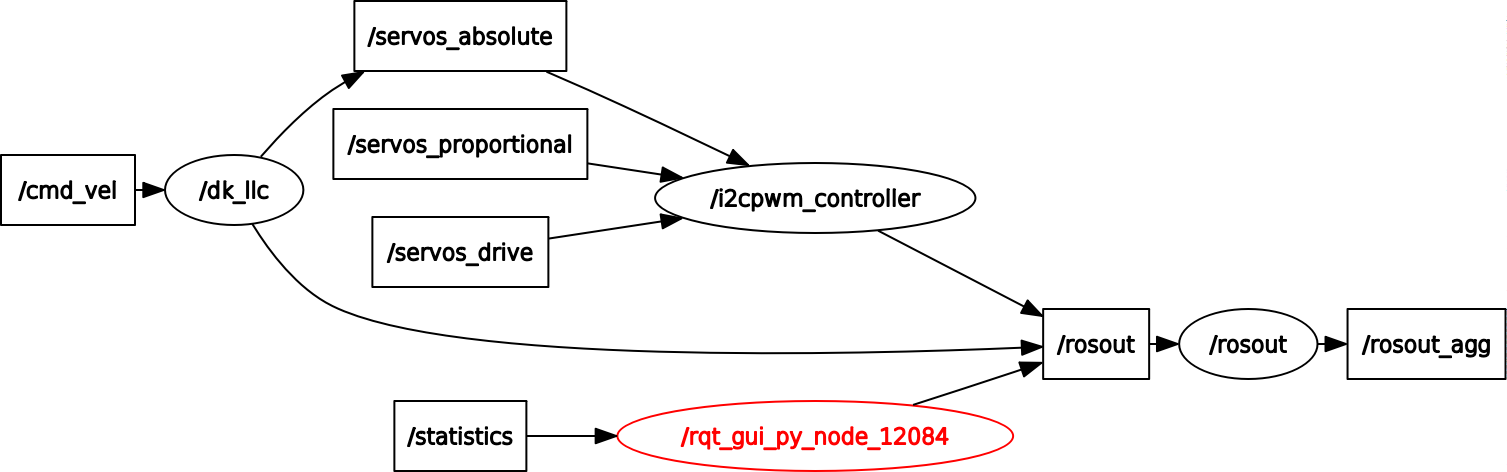
\includegraphics[width=9cm]{img/rosgraph.png}
	\caption{Übersicht der ROS Elemente}
	\label{rosgraph}
\end{figure}

Treu nach den Prinzipien von ROS besteht die Software aus vielen ROS Nodes, welche als Oval dargestellt werden. 
Jede Node erledigt kleine Aufgaben und kann als Subscriber und/oder Publisher fungieren.
Die Kommunikation zwischen Subscriber und Publisher erfolgt durch ROS Messages (Nachrichten).
Diese werden durch verschiedene Topics — werden als Rechteck dargestellt — kommuniziert.
Die Topics kann man als Kanäle für Nachrichten betrachten.

Folgende Nodes befinden sich im Softwaresystem:
\begin{itemize}
	\item /rosout (Master)
	\item /teleop\_twist\_keyboard (Fernsteuerung)
	\item /donkey\_llc (Hardwarenahe Steuerung)
	\item /ic2pwm\_board\_node (Bibliothek und Node zum Ansprechen des I2C Protokolls und deren Verbindung mit ROS)
	\item serial\_node.py (Publisher der Utraschallsensordaten)
\end{itemize}

Die zuvor genannten Nodes sind durch Topics miteinander verbunden und tauschen untereinander Nachrichten aus.
Folgende Topics befinden sich im Softwaresystem:
\begin{itemize}
	\item /cmd\_vel (command velocity, die Beschleunigungssteuerung)
	\item /servos\_absolute (Steuerung des Servos mit absoluten Impulsstart- und Stoppwerten)
	\item /servos\_proportional (Motorsteuerung für Geschwindigkeitsteuerung des Servos in seinem Bewegungsbereich)
	\item /servos\_drive (Lenken, Umwandlung der Berechnungen von Linear- und Winkeldaten in Servoantriebsdaten)
	\item /rosout (Standard ROS Output)
	\item /rangeMsg\_topic (Datenübertragung der Ultraschallsensordaten)
\end{itemize}

%----------------------------------------------------------------
% Je nach Formatierung wird dies verändert werden dürfen und der pagebreak entfernt
\pagebreak
\subsubsection{Launchreihenfolge}%heike

Dieses Kapitel ist eine Einleitung zum Starten der ROS Nodes und den hierbei zu beachtenden Punkten.

% Weitere Knoten werden noch folgen
\begin{lstlisting}[label={list:first},caption=Sample rosBash code.]
	# Network ubiquityrobot03B
	# connect via SSH
	ssh ubuntu@10.42.0.1
	# enter password

	# 1. Console - on Raspberry Pi
	# Login via SSH
	cd catkin_ws/Robotic_AI_student_project/
	source devel/setup.bash
	rosrun i2cpwm_board i2cpwm_board

	# 2. Console - on Raspberry Pi
	# Login via SSH
	cd catkin_ws/Robotic_AI_student_project/
	source devel/setup.bash
	rosrun donkey_car low_level_control.py

	# 3. Console - on Laptop 
	export ROS_MASTER_URI=http://ubiquityrobot.local:11311
	export ROS_IP=$(hostname -I)
	cd catkin_ws/Robotic_AI_student_project/
	source devel/setup.bash
	rosrun teleop_twist_keyboard teleop_twist_keyboard.py

	# 4. Console - on Raspberry Pi
	# Login via SSH
	rosrun rosserial_python serial_node.py /dev/ttyACM0

	# 5. Console - on Laptop
	export ROS_MASTER_URI=http://ubiquityrobot.local:11311
	export ROS_IP=$(hostname -I)
	rostopic echo rangeMsg_topic
\end{lstlisting}
%----------------------------------------------------------------

\section{Praktische Projektdurchführung}

%----------------------------------------------------------------

\subsection{Hardwareaufbau}%Heike 
In diesem Kapitel beschreiben wir den Hardwareaufbau des rosBerry.
Hierfür werden wir die einzelnen verwendeten Hardwarekomponenten — deren Modell und Funktion — vorstellen.

Zuerst bilden wir die Verbindungen der Hardwarekomponenten untereinander ab, wie in Abbildung \ref{Hardwarekomponenten} zu sehen.

\begin{figure}[!ht]
	\centering
	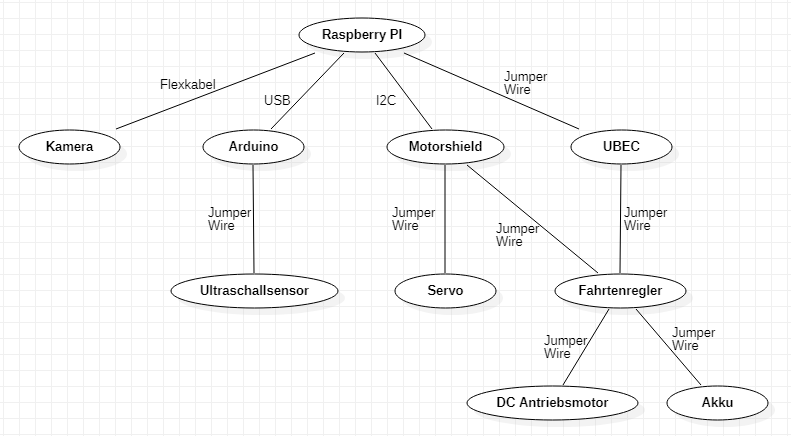
\includegraphics[width=9cm]{img/Hardwarekomponenten.PNG}
	\caption{Verbindungen der Hardwarekomponenten im rosBerry}
	\label{Hardwarekomponenten}
\end{figure}

Wie aus der Abbildung \ref{Hardwarekomponenten} zu erkennen, ist die meiste Hardware mit Jumper Wire verbunden.
Ausnahmen der Anschlüsse bilden die Verbindungen des Raspberry Pis zur Kamera (Flexkabel), zum Arduino (USB) und zum Motorshield (I2C).
\\

Als Nächstes wird rosBerry mit den Hardwaremodellen vorgestellt.
\\
\begin{figure}[!ht]
	\centering
	\includegraphics[width=9cm]{img/RosBerryGesamt.png}
	\caption{Gerüst rosBerry}
	\label{rosBerryGesamt}
\end{figure}

Die verwendete Hardware ist in Abbildung \ref{rosBerryGesamt} mit Nummern versehen.
Auf jede dieser Nummern wird referenziert und die Hardware mit Modell und Funktion aufgelistet.

\begin{enumerate}
	\item Der DC Antriebsmotor — Modell Tamiya Mabuchi RS 540 SH — steuert alle vier Reifen des rosBerry an.
	Ohne ihn wird der Roboter nicht in Bewegung kommen.
	\item Neben dem DC Antriebsmotor befindet sich ein Fahrtenregler, Modell BORSTI 1/10 BRUSHED-ESC 45A.
	Dieser erhält vom Motorshield ein PWM Signal, welches er verstärkt.
	Das verstärkte PWM Signal wird anschließend in Geschwindigkeit umgesetzt und an den DC Antriebsmotor weitergeleitet.
	\item Der UBEC — Modell HWBEC Hobbywing 3A 5V 6V max 5A — wird eingebaut, um den Raspberry Pi mit 5 Volt zu versorgen.
	Ohne den UBEC würde der Raspberry Pi aufgrund der höheren elektrischen Spannung beschädigt werden.
	\item Der Servo — Modell Amewi AMX Racing 4806HB — bekommt vom Motorshield ein PWM Signal übermittelt.
	Nach dem PWM Signal richten sich die beiden Reifen aus und ermöglichen eine Fahrtrichtung.
	Dadurch ist rosBerry in der Lage rechts/links Kurven sowie geradeaus zu fahren.
	\item Der Akku dient dazu, die Stromversorgung des Roboters zu sichern.
	Dieser liefert 7 Volt und versorgt die weitere Hardware mit Strom.
	\item Der Motorshield — Modell Adafruit 16-Channel 12-bit PWM/Servo Driver-I2C interface PCA9685 — wird für die Geschwindigkeit und die Richtung der Reifen eingesetzt.
	Hierzu erzeugt der Motorshield zwei PWM Signale.
	Das 1. PWM Signal wird an den Servo übermittelt, um den Servo in die gewünschte Position einzustellen.
	Das 2. PWM Signal wird erzeugt und zum Fahrtenregler gesendet.
	Dieses wird zur Einstellung der Geschwindigkeit verwendet.
	\item Der Raspberry Pi 3.b+ ist das Herzstück des rosBerry.
	Auf ihn läuft zum einem ROS und zum anderen die Software des Roboters, welche im Kapitel ROS Knoten Software Architektur vorgestellt wurde.
	Über eine I2C-Schnittstelle werden Daten an den Motorshield übertragen.
	Die Daten geben an, wie das PWM Signal auszusehen hat.
	\item Der Arduino UNO REV 3 steuert einen Ultraschallsensor an und erzeugt einen ROS Knoten (Publisher).
	Innerhalb des Programms wird das Signal des Sensors in Meter umgewandelt und in eine Range Message gespeichert.
	Die Range Message namens rangeMsg wird an das Topic rangeMsg\_topic übermittelt.
	Ein Subscriber — der auf dem Raspberry Pi läuft — subscribed das Topic und erhält regelmäßig Sensordaten über die Reichweite.
	
	\begin{figure}[!ht]
		\centering
		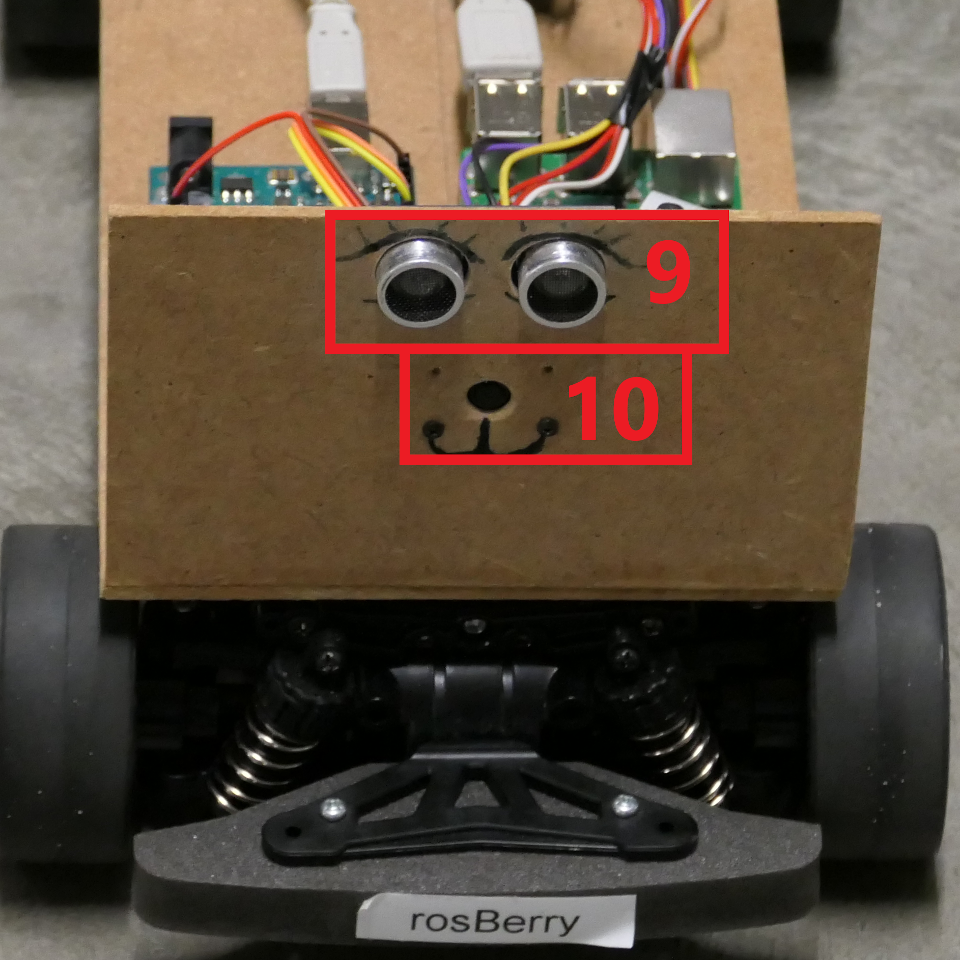
\includegraphics[width=5.5cm]{img/RosBerryWeitere.png}
		\caption{Weitere Hardwareelemente}
		\label{rosBerryWeitere}
	\end{figure}
	\item Der Ultraschallsensor — Modell HC-SR04 — wird zum rechtzeitigen Erkennen eines kommenden Hindernisses eingesetzt.
	Dieser hat eine maximale Reichweite von 4 Meter, jedoch haben wir uns für das Projekt auf eine Reichweite von 2 Meter geeinigt.
	Alle x Sekunden sendet dieser ein Signal und verarbeitet dieses.
	\item Die Kamera — Modell 5 MP — ist durch ein Flexkabel an den Raspberry Pi angeschlossen.
	Diese versorgt die KI mit Bildern, welche einen Marker sucht und findet.
\end{enumerate}

%----------------------------------------------------------------


\section{Autonomes Verhalten durch Künstliche Intelligenz}	%mary

Ziel des KI Teils des Projektes besteht darin, dem Roboter beizubringen einem optischen Marker zu folgen.
Dazu muss er erst einmal das Symbol erkennen, dann herausfinden in welcher Richtung sich der Marker befindet.
Danach erst kann er auf den Marker zufahren.
\\

Der schwierigste Teil der Aufgabe besteht darin, den Marker zuverlässig in unterschiedlichen Umgebungen zu erkennen.

\subsection{Erster Ansatz für das Neuronale Netz}	%steffen ? mary?
%netzaufbau am anfang
Der erste Entwurf unseres Neuronalen Netzes war stark angelehnt an F. Grovers Beispielnetz aus \glqq Artificial Intelligence for Robotics\grqq \cite{b1}.Wie in der Vorlage erstellen wir ein sequentielles Modell mithilfe von Keras.

Die erste Schicht stellt ein convolution layer mit 20 convolutions dar, wovon jede ein Merkmal des Eingangsbildes isolieren soll.
Die Größe setzen wir auf 5x5, betrachten also zwei benachbarte Pixel in jede Richtung.
Selbstverständlich muss dafür auch ein Padding hinzugefügt werden, damit das Verfahren auch am Bildrand funktioniert. 

Zudem wird noch eine Aktivierungsfunktion benötigt, hierfür nutzen wir die ReLU-Funktion, die nur positive Werte zulässt und negative Werte durch den Wert 0 ersetzt.
Diese Aktivierungsfunktion ergibt deshalb Sinn, da das Ergebnis als Farbe dargestellt werden und deshalb einen Wert zwischen 0 und 1 annehmen soll.
Ein Wert unter Null wäre hier unsinnig.

\begin{lstlisting}[label={list:model_1_1},caption=Sequentielles Modell und erste Schicht]
	model = Sequential()
	inputShape = (height, width, depth)

	model.add(Conv2D(20, (5, 5), padding="same", input_shape=inputShape))
	model.add(Activation("relu"))
\end{lstlisting}

Die zweite Schicht ist ein maxpooling layer, bei dem wir jeweils 2x2 Pixel nehmen und danach 2x2 Pixel weiterrücken um keine Überlappungen zu haben.
Das Ergebnis ist ein Bild in ¼ der originalen Größe: aus 640x480px wird 320x240px, aus 128x128px 64x64px usw.

Direkt darauf folgt ein weiteres convolution layer mit der doppelten Anzahl an convolutions — 40 statt vorher 20 — um mehr Mermale zu identifizieren.
Durch das vorher durchgeführte maxpooling werden nun andere, größere Merkmale erkannt.
Ebenfalls nutzen wir wieder dieselbe ReLU Aktivierungsfunktion, aus denselben Gründen wie in der ersten Schicht.

\begin{lstlisting}[label={list:model_1_2},caption=Modell: zweite und dritte Schicht]
	model.add(MaxPooling2D(pool_size=(2, 2), strides=(2, 2)))

	model.add(Conv2D(40, (5, 5), padding="same"))
	model.add(Activation("relu"))
\end{lstlisting}

Schicht vier besteht erneut aus einem maxpooling layer, ebenfalls um nochmals größere Merkmale zu erkennen.
Aus einem 640x480px großen Bild wird nun 160x120px, aus 128x128px sogar nur noch 32x32px.

Darauf folgt nun eine Schicht, die vorher noch nicht im Neuronalen Netz vorkam:
Zuerst werden die dreidimensionalen Bildinformationen mit der Funktion Flatten() in ein eindimensionales Array geplättet, bevor wir eine vollverknüpfte Schicht mittels Dense(500) hinzufügen.
Erneut nutzen wir die ReLU Aktivierungsfunktion, aus bekannten Gründen.

\begin{lstlisting}[label={list:model_1_3},caption=Modell: vierte und fünfte Schicht]
	model.add(MaxPooling2D(pool_size=(2, 2), strides=(2, 2)))

	model.add(Flatten())
	model.add(Dense(500))
	model.add(Activation("relu"))
\end{lstlisting}

Abschließend benötigen wir zwei Neuronen für die beiden Ausgangswerte "Marker" und "kein Marker".
Zur Aktivierung nutzen wir die Softmax-Funktion, die auch normalisierte Exponentialfunktion genannt wird.
Sie transformiert mehrdimensionale Vektoren in einen Wertebereich zwischen 0 und 1, wobei alle Komponenten zusammen 1 ergeben müssen, das heißt wenn "Marker" einen Wert von 0,65 hat, muss "kein Marker" einen Wert von 0,35 haben. 
Die Funktion kann durchaus für mehr als zwei Ausgangswerte genutzt werden, für unseren Anwendungsfall werden jedoch nicht mehr Ausgangswerte benötigt.

\begin{lstlisting}[label={list:model_1_4},caption=Modell: finale sechste Schicht]
	model.add(Dense(2))
	model.add(Activation("softmax"))
\end{lstlisting}

\subsubsection{Erste Auswertung der Ergebnisse}	%steffen? 
%wiso war das scheisse 
%weil wir einfach das Beispiel aus dem Buch kopiert haben…

\subsection{Schritte zur Verbesserung der Erkennungsrate} %mary
%was haben wir dann gemacht 


\begin{figure}[!h]
	\centering
	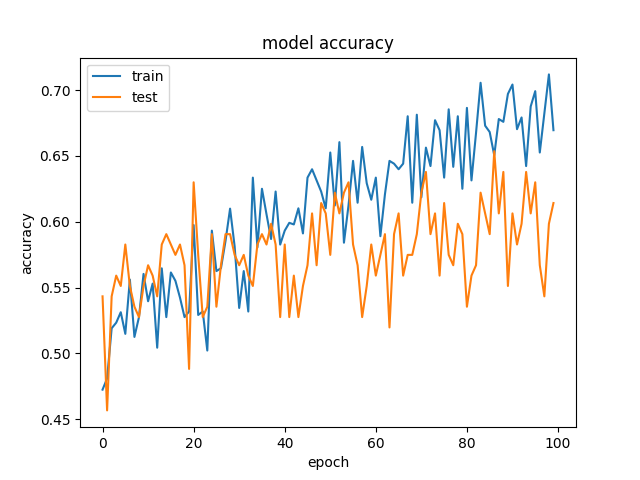
\includegraphics[width=9cm]{img/160x120:100@32_accuracy.png}
	\caption{erster Durchlauf}
	\label{Initiales Ergebnis}
\end{figure}
Beim ersten Durchlauf des Neuronalen Netzes war die Erkennungsrate des Markers 57\%. Dieses Ergebnis ist bei einer 50/50 Chance kaum besser als Raten.\\

Die Schritte von  \glqq Learn Keras for Deep Neural Networkss\grqq  \cite{b3} zum verbessern des Designs von Neurnalen Netzen wurden zur verbesserung der Trainignsergebnisse verwedet. 

\cite{b3}  Rät dazu mit einer kleinen Architektur anfangen das bedeutet wenige Schichten und wenige Neuronen. Es liegt nahe das kleine Architekturen Ressourcen schonender sind als grosse Architekturen. Dieser ansatz erscheint sinnvoll da Steigende Resourcenanforderngen bei gleichbleibender Hardware zu steigender Rechenzeit pro Epoche bedeuten. \\

Das Netz nutzte anfangs nur eine Auflösung von 128x128 Pixel und 100 Epochen. Da jedes einzelne Pixel eine Eingangsneurone wird, ist anzunehmen, dass die geringe Auflösung im Buch gewählt wurde, um Rechenleistung zu sparen. \\

\begin{figure}[!h]
	\centering
	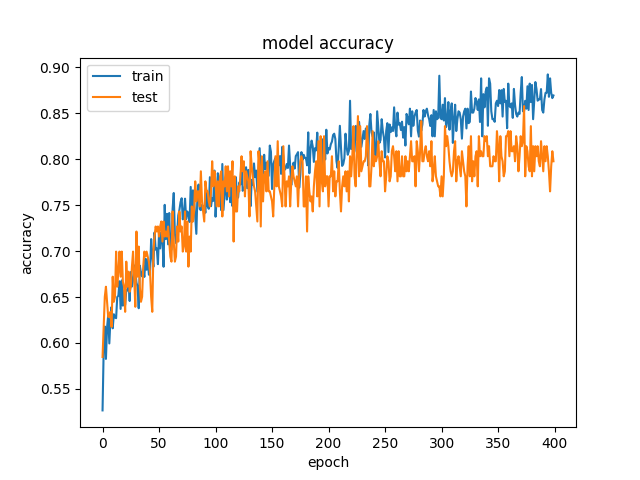
\includegraphics[width=9cm]{img/213x160:400@32_accuracy.png}
	\caption{overfitting}
	\label{Overfitt }
\end{figure}

\cite{b3} Rät die Anzahl an Neuronen pro Schicht erhöhen, wenn Anfangs kein befriedigenden Ergebnisse erzieht werden.
Bei voller Bildauflösung von 640x480 Pixel erweist sich das Neuronale Netz auf der Hardware eines handelsüblichen Laptops als nicht mehr lauffähig. Für weitere Durchläufe wurden die nächsten Versuche auf einer Workstation mit mehr Grafkikkarten und Deutlich mehr RAM gemacht. Die Erkennungsrate stieg bei größerer Auflösung und mehr Durchläufen tatsächlich auf über 80\%. Damit vergrösserte sich jedoch das Modell (die Gewichte der KI) auf über ein Gigabyte. Ein so großes Modell kann nicht zeitnahe auf einem Raspberry Pie angewedet werden, da es nicht mehr in den RAM passt. Auch auf Standart Laptops ist zu erwarten das ein größeres Modell echt zeit Berechnungen erschwert. \\


Um mit einer höhreren Auflösung trainiren zu können wurden die nächsten Trainingseinheiten auf einem performateren Server durchgeführt. Der zusätzliche Arbeitsspeicher und die Grafikarten bringen bei einer aktivierung der CUDA beschleunigung einen grossen Geschwikdikeitszuwachs . \\

Ein weiteres Problem das zu Tage trat war das Overfitting. Das Modell entwickelte sich gut auf Trainingsdaten, schnitt jedoch deutlich schlechter bei Testdaten ab, mit denen es nicht trainiert hatte. Die Kurven liefen bei mehr als 200 Epochen weit auseinander.\\


Weiterhin Rät \cite{b3} mehr Schichen benutzen, Beispielsweise abwechselnd eine Dichte schicht( dense layer) und eine Dropout Schicht.

Dropout Schichten im Neuronalen Netz verbesserten das Overfitting Problem. Somit waren mehr Trainingsläufe ohne overfitting möglich. Das neuronale Netz erreichte so werte von rund 85\%. \\

Das Modell das TensorFlow bei voller Auflösung oder 307200 Eingangsneuronen erstellt ist über ein Gigabyte groß. Je größer das Modell ist, des do unwahrscheinlicher das ein Raspberry Pi das Modell in absehbarer Zeit auf ein Bild anwenden kann. Somit erwies sich der Ansatz einfach die Auflösung zu erhöhen als nicht  zielführend für den Anwendungsfall. \\

Das Modell musste also kleiner werden ohne wesentliches Overfitting. Diese Ziehl wurde durch die Kombination von Dropoutschichten, mehr Durchläufen und kleinerer Pixelanzahl erreicht. \\

\cite{b3} Rät weiterhin, die Daten neu analysieren, wenn eine weitere Steigerung der Anzahl an Schichten und der Neuronen keine weitere Steigerung der Erkennungsrate bringt. Es wurden als Bilder mit sehr geringem Kontrast aussortiert, extrem Dunkle Bilder sowie Bilder auf denen der Marker sehr weit entfernt war. Sie wurden durch Bessere Daten ersetzt. (neue Bilder wurden angefertigt jeweils mit und Ohne Marker) Dieser Schritt verursachte eine Merkliche Verbesserung des Trainingsergebnis.
\\


\begin{figure}[!h]
	\centering
	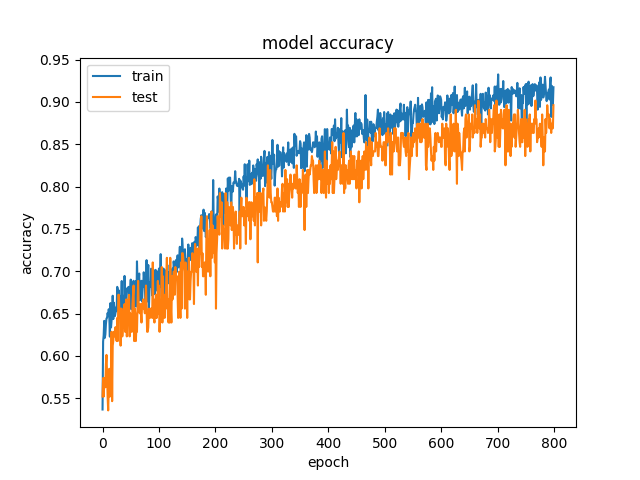
\includegraphics[width=9cm]{img/213x160:800@32:0_accuracy.png}
	\caption{Enderge ergebnis}
	\label{end Ergenisse }
\end{figure}

Alle weiteren versucht das Model weiter zu verfeinern scheiterten. Es ist zu vermuten das der Datensatz zu klein war für die komplexität des Models. Eine weitere möglichkeit ist das die Grenzen der Optimierer ADAM und Stochastic Gradient Descent erreicht waren. 
\begin{figure}[!h]
	\centering
	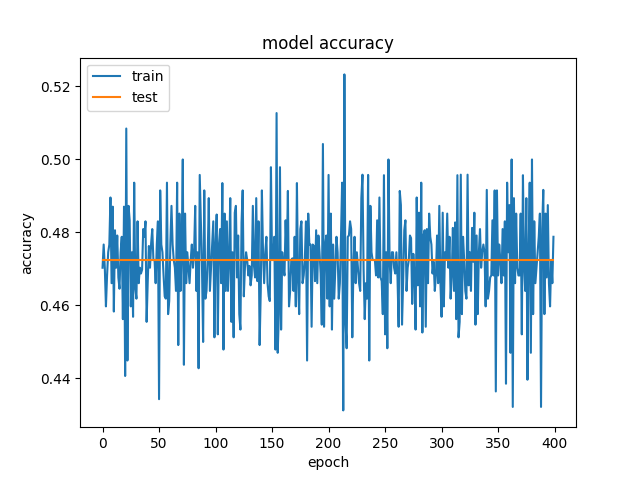
\includegraphics[width=9cm]{img/480x360:400@32_accuracy.png}
	\caption{Kein sichtbarer Trainingserfolg}
	\label{erfolgloos }
\end{figure}


\subsection{Anwendung des Trainingsmodells} %steffen
%mach ich! ~steffen
%bild teilen
%bild analysieren
%  entscheidung treffen, rechts, links geradeaus oder rückwärtz
\subsection {Auswertung des Verhalten des Roboters}	% mary? %steffen? %heike?
%macht er irgendwas sinnvolles? ist er klüger als eine eintagsfliege

\begin{comment}	%  how-to formeln 
\begin{equation}
a+b=\gamma\label{eq}
\end{equation}
\end{comment}
\begin{comment}
\paragraph{Positioning Figures and Tables} 
Use the abbreviation 
``Fig.~\ref{fig}'', even at the beginning of a sentence.

\begin{table}[htbp]
\caption{Table Type Styles}
\begin{center}
\begin{tabular}{|c|c|c|c|}
\hline
\textbf{Table}&\multicolumn{3}{|c|}{\textbf{Table Column Head}} \\
\cline{2-4} 
\textbf{Head} & \textbf{\textit{Table column subhead}}& \textbf{\textit{Subhead}}& \textbf{\textit{Subhead}} \\
\hline
copy& More table copy$^{\mathrm{a}}$& &  \\
\hline
\multicolumn{4}{l}{$^{\mathrm{a}}$Sample of a Table footnote.}
\end{tabular}
\label{tab1}
\end{center}
\end{table}

\begin{figure}[htbp]
\centerline{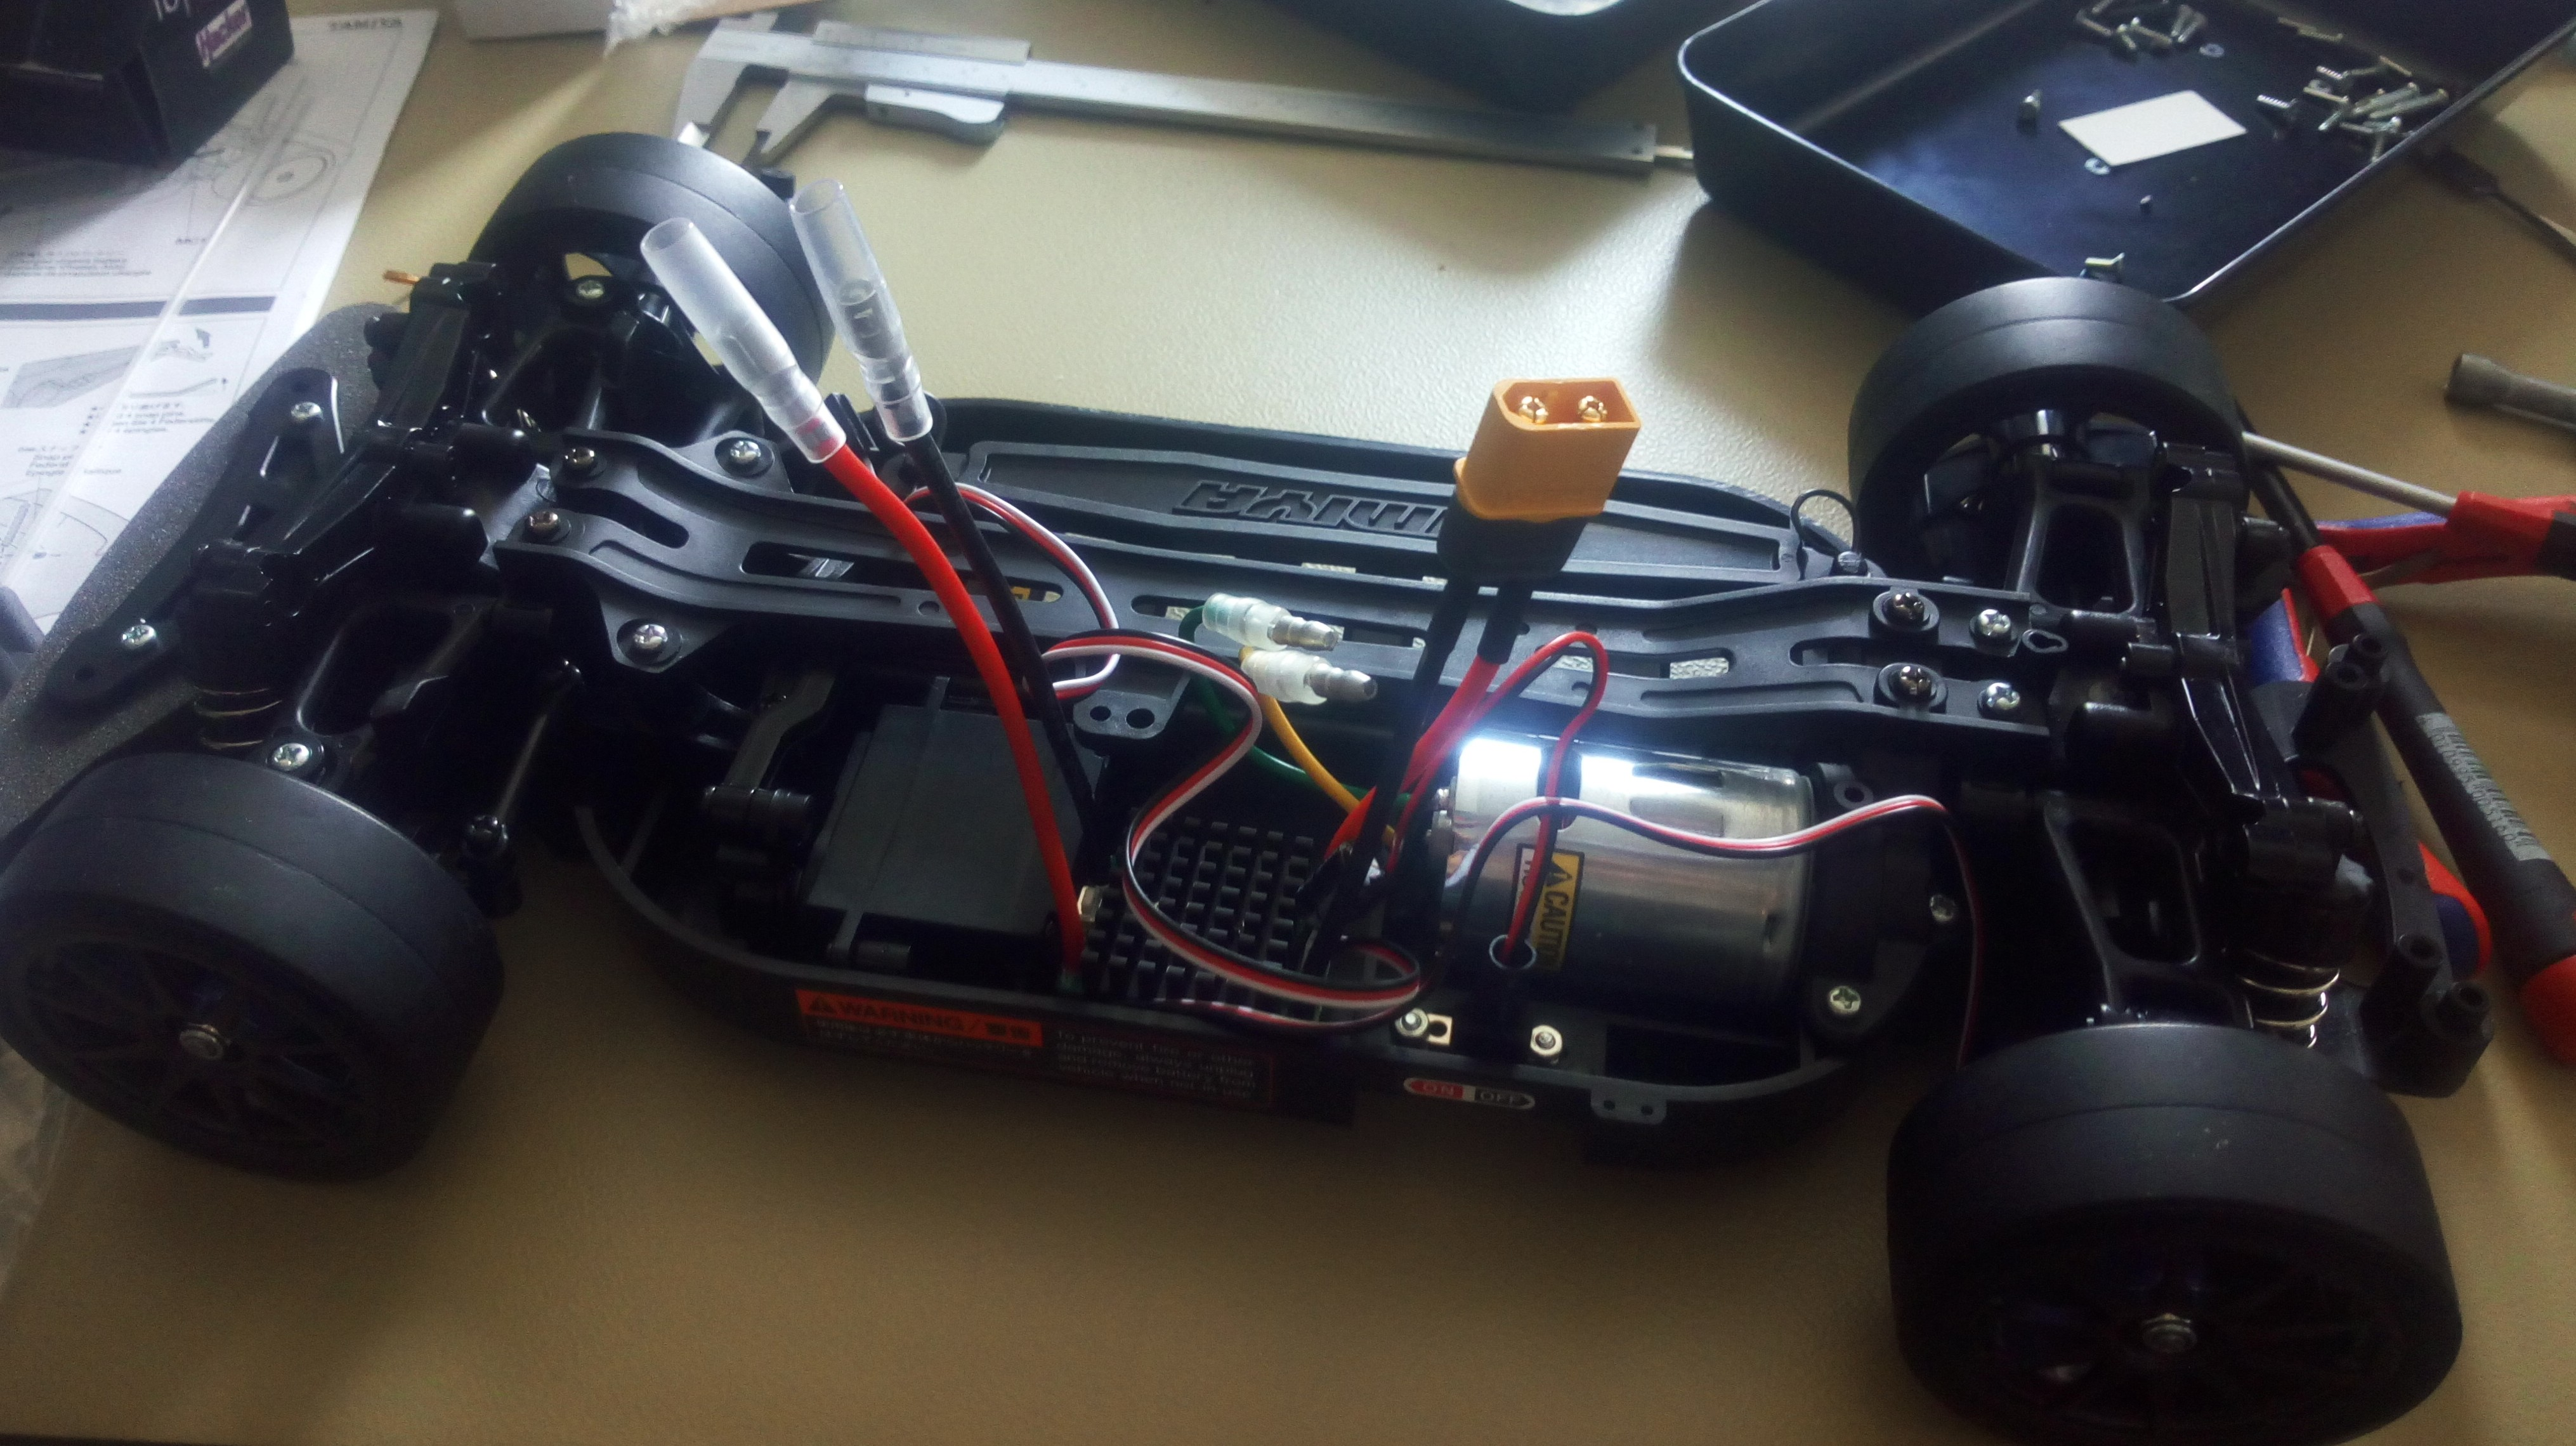
\includegraphics{img/car_body.jpg}}
\caption{Example of a figure caption.}
\label{fig}
\end{figure}
\end{comment}


%\section*{Acknowledgment}
% wollen wir unseren profs danken, weil mehr GPU und RAM? 

% wissenschaftliche zitate gehen so \cite{b1}. 


%Francis X. Govers - Artificial Intelligence for Robotics-Packt Publishing (2018).pdf
\begin{thebibliography}{00}
	\bibitem{b1}Francis X. Govers , Artificial Intelligence for Robotics, Packt Publishing ,2018
	\bibitem{b2}Amanda Decker , Bachelor Arbeit, Hochschule Mannheim ,2019
	\bibitem{b3}Learn Keras for Deep Neural Networks, Jojo Moolayil apress, 2019
\end{thebibliography}


\end{document}
